\documentclass[12pt,a4paper]{article}

\usepackage[utf8]{inputenc}
\usepackage{geometry}
\usepackage{graphicx}
\usepackage{float}
\usepackage{array}
\usepackage{booktabs}
\usepackage{longtable}
\usepackage{caption}
\usepackage{subcaption}
\usepackage{hyperref}
\usepackage{enumitem}
\usepackage{xcolor}
\usepackage{amsmath}

\geometry{margin=2.5cm}
\setlength{\parskip}{0.7em}
\setlength{\parindent}{0pt}
\renewcommand{\labelitemi}{--}
\renewcommand{\labelitemii}{--}
\captionsetup{font=small,labelfont=bf}
\hypersetup{
    colorlinks=true,
    linkcolor=blue!50!black,
    urlcolor=blue!60!black,
    pdftitle={Documentación Práctica 3 - Organización Computacional},
    pdfauthor={Grupo 21}
}

\title{Documentación Técnica\\Práctica 3 - Organización Computacional}
\author{Grupo 21}
\date{17 de abril de 2026}

\begin{document}

\begin{titlepage}
    \centering
    \vspace*{1.5cm}
    
\includegraphics[width=0.23\textwidth]{assets/usac_logo.png}\par\vspace{1cm}
    {\scshape\LARGE Universidad de San Carlos de Guatemala \par}
    \vspace{0.4cm}
    {\scshape\Large Facultad de Ingeniería \par}
    \vspace{0.2cm}
    {\scshape\large Escuela de Ciencias y Sistemas \par}
    \vspace{1.8cm}
    {\Huge\bfseries Práctica 3\\[0.2cm] Organización Computacional\par}
    \vspace{0.8cm}
    {\Large Documentación del \textit{Carrusel Automatizado con Control de Acceso Seguro}\par}
    \vspace{1cm}
    \begin{tabular}{|c|p{8.2cm}|}
        \hline
        \textbf{Carnet} & \textbf{Integrante} \\
        \hline
        202406918 & Claudia Maribel Tigüilá Tecum \\
        \hline
        202403929 & Emiliana Elizabeth Pú Lara \\
        \hline
        202300476 & Alex Ricardo Castañeda Rodríguez \\
        \hline
        201904522 & Byron Manuel Hernández López \\
        \hline
    \end{tabular}
    \vfill
    {\large Grupo 21\par}
    {\large Abril de 2026\par}
    \vfill
\end{titlepage}

\tableofcontents
\newpage

\section{Introducción}
La práctica 3 consistió en diseñar, simular e implementar un carrusel automatizado con control de acceso seguro. El sistema debía resolver dos necesidades de forma integrada: restringir la activación del carrusel a usuarios autorizados mediante una contraseña digital de 4 bits y, al mismo tiempo, coordinar el movimiento del motor, la señalización luminosa y la visualización temporal durante cada ciclo de operación.

La solución se dividió en módulos independientes para facilitar el análisis, el cableado y la depuración del circuito. La autenticación se resolvió con flip-flops, comparador de 4 bits, lógica de validación y un contador de errores con alarma. El movimiento del carrusel se separó en una etapa de control de potencia con puente H y una etapa de temporización apoyada por un Arduino que únicamente genera pulsos de reloj y señales de dirección. De esta forma se respetó la restricción del enunciado: el Arduino no reemplaza la lógica digital central, sino que actúa como apoyo para la sincronización temporal del sistema.

La presente documentación toma como base la estructura formal utilizada en la práctica anterior, pero adapta el contenido técnico a los requerimientos específicos de esta práctica. Además de describir el funcionamiento general, se detalla la lógica seguida en cada módulo y se incorporan capturas del diseño en Proteus junto con fotografías del armado físico realizado por el grupo.

\section{Objetivos}

\subsection{Objetivo general}
Diseñar e implementar un carrusel automatizado que integre autenticación de 4 bits, conteo de errores, alarma de seguridad, control bidireccional de motor DC y visualización temporal mediante displays de siete segmentos.

\subsection{Objetivos específicos}
\begin{itemize}[leftmargin=1.2cm]
    \item Almacenar una contraseña de 4 bits en flip-flops tipo D y compararla contra una entrada de usuario independiente.
    \item Detectar intentos fallidos, contarlos hasta tres eventos y activar una alarma persistente hasta ingresar la contraseña correcta.
    \item Generar una secuencia de operación de 15 segundos en sentido de avance y 10 segundos en sentido contrario.
    \item Controlar un motor DC mediante un puente H discreto y asociar el sentido de giro con indicadores visuales.
    \item Mostrar en displays de siete segmentos el tiempo activo del sistema y el número de errores acumulados.
\end{itemize}

\section{Resumen del enunciado}
El enunciado solicita una maqueta funcional de carrusel con acceso seguro. La contraseña debe almacenarse con flip-flops tipo D y compararse con la entrada del usuario por medio de un comparador de 4 bits. Si el intento es incorrecto, se incrementa un contador de errores mostrado en display; al alcanzar tres errores, se activa una alarma. Cuando la contraseña es correcta, el sistema habilita el movimiento del carrusel, reinicia el contador de errores y apaga la alarma.

Una vez autenticado el usuario, el motor debe girar en una primera dirección durante 15 segundos con LED verde y contador ascendente. Después debe cambiar a la dirección contraria durante 10 segundos con LED rojo y contador descendente. La implementación debía entregarse tanto en Proteus como en maqueta física, acompañada de documentación técnica completa.

\section{Arquitectura general del sistema}
El proyecto se organizó en cinco bloques principales:
\begin{enumerate}
    \item Registro y validación de contraseña.
    \item Contador de errores y alarma.
    \item Temporización y secuencia de operación.
    \item Multiplexación y visualización en displays.
    \item Control del motor DC y estructura física del carrusel.
\end{enumerate}

\begin{table}[H]
    \centering
    \caption{Resumen funcional de módulos implementados.}
    \small
    \begin{tabular}{p{3.2cm}p{3.4cm}p{3.2cm}p{4.2cm}}
        \toprule
        \textbf{Módulo} & \textbf{Integrados o elementos} & \textbf{Entradas principales} & \textbf{Función} \\
        \midrule
        Unidad de control & Arduino Uno & AUTH\_OK, reloj interno & Genera pulsos de 1 Hz y controla dirección del motor \\
        Registro de contraseña & 74LS174, switches, pulsadores & SW de memoria, CLK\_MEM, RESET & Guarda la contraseña de 4 bits \\
        Comparación y habilitación & 74LS85, 74LS74 & MEM[3:0], USER[3:0], VALIDATE & Valida el acceso y memoriza la habilitación \\
        Contador de errores & 74LS74, 74LS20, 74LS04, 74LS48 & ERROR, RESET, MATCH & Cuenta intentos fallidos y activa alarma al llegar a 3 \\
        Temporización & 74LS74, 74LS08, 74LS32, Arduino & CLK\_UP, CLK\_DOWN & Genera conteos de 0 a 15 y de 10 a 0 \\
        Visualización de tiempo & 74LS157, 74LS283, 74LS48, displays & Q[3:0], Y[3:0], fase & Selecciona el conteo activo y lo adapta a BCD \\
        Puente H y LEDs & 2N2222A, 1N4007, motor DC, LEDs & IN1, IN2 & Invierte el giro del motor y muestra el sentido activo \\
        \bottomrule
    \end{tabular}
\end{table}

\subsection{Secuencia de operación}
La lógica completa del carrusel puede resumirse así:
\begin{enumerate}
    \item Se define una contraseña de 4 bits mediante el bloque de memoria.
    \item El usuario ingresa otra combinación de 4 bits y presiona el botón de validación.
    \item Si la comparación es correcta, se activa la señal \texttt{AUTH\_OK}; si es incorrecta, se genera un pulso \texttt{ERROR}.
    \item El contador de errores incrementa hasta 3; en ese estado se mantiene la alarma encendida y se deshabilita el movimiento.
    \item Cuando \texttt{AUTH\_OK} está activa, el Arduino genera 15 pulsos para el contador ascendente y hace girar el motor en una dirección.
    \item Al terminar esos 15 segundos, cambia de dirección, emite 10 pulsos para el contador descendente y conmuta el LED rojo.
    \item Al finalizar el ciclo, el sistema detiene el motor y queda listo para una nueva autenticación.
\end{enumerate}

\section{Funciones booleanas y mapas de Karnaugh}
Aunque el sistema completo combina lógica secuencial y combinacional, varios bloques críticos pueden describirse con funciones booleanas simples. Estas expresiones fueron útiles para decidir qué compuertas eran necesarias y para verificar la coherencia del diseño visto en Proteus.

\subsection{Generación de pulso de error}
Si \texttt{MATCH} representa coincidencia entre contraseña almacenada y entrada de usuario, y \texttt{VALIDATE} representa el pulso del botón de ingreso, entonces un error solo debe producirse cuando el usuario intenta validar y la comparación es falsa:

\[
ERROR = VALIDATE \cdot \overline{MATCH}
\]

\begin{table}[H]
    \centering
    \caption{Mapa de Karnaugh para la señal \texttt{ERROR}.}
    \begin{tabular}{c|cc}
        \toprule
        \textbf{VALIDATE $\backslash$ MATCH} & 0 & 1 \\
        \midrule
        0 & 0 & 0 \\
        1 & 1 & 0 \\
        \bottomrule
    \end{tabular}
\end{table}

La simplificación no puede reducirse más: el único mintermino activo es $VALIDATE \cdot \overline{MATCH}$.

\subsection{Activación de alarma}
El contador de errores usa dos bits visibles como estado interno. La alarma se dispara cuando ambos bits están en uno, es decir, al alcanzar el estado binario 3:

\[
ALRM = BIT1 \cdot BIT0
\]

\begin{table}[H]
    \centering
    \caption{Mapa de Karnaugh para la alarma de 3 errores.}
    \begin{tabular}{c|cc}
        \toprule
        \textbf{BIT1 $\backslash$ BIT0} & 0 & 1 \\
        \midrule
        0 & 0 & 0 \\
        1 & 0 & 1 \\
        \bottomrule
    \end{tabular}
\end{table}

Esta misma salida se invierte para generar la señal de habilitación general:

\[
ENABLE = \overline{ALRM}
\]

\subsection{Señales de dirección del motor}
La etapa de potencia requiere dos líneas excluyentes:

\[
H1 = AUTH\_OK \cdot FASE\_VERDE
\]
\[
H2 = AUTH\_OK \cdot FASE\_ROJA
\]

donde \texttt{FASE\_VERDE} es la primera ventana de 15 segundos y \texttt{FASE\_ROJA} es la segunda ventana de 10 segundos. La tabla de comportamiento es la siguiente:

\begin{table}[H]
    \centering
    \caption{Tabla funcional del puente H.}
    \begin{tabular}{c c c p{5.4cm}}
        \toprule
        \textbf{AUTH\_OK} & \textbf{H1} & \textbf{H2} & \textbf{Efecto} \\
        \midrule
        0 & 0 & 0 & Motor detenido \\
        1 & 1 & 0 & Giro en primera dirección, LED verde activo \\
        1 & 0 & 1 & Giro en dirección contraria, LED rojo activo \\
        1 & 1 & 1 & Estado no permitido, se evita en la lógica de control \\
        \bottomrule
    \end{tabular}
\end{table}

\subsection{Lógica de visualización}
En la sección de tiempo fue necesario seleccionar entre dos contadores: el ascendente de 0 a 15 y el descendente de 10 a 0. Para ello se usó multiplexación, de forma que únicamente un conjunto de bits llegue al bloque BCD en cada fase. La idea lógica es:

\[
DISPLAY = \begin{cases}
Q[3:0], & \text{fase verde} \\
Y[3:0], & \text{fase roja}
\end{cases}
\]

Además, se generó una señal de decenas para mostrar correctamente el valor 10 durante la fase descendente y el paso a decenas en el ascendente cuando el conteo supera 9.

\section{Diseño del circuito por módulos}

\subsection{Unidad de control con Arduino}
El Arduino no realiza comparación de contraseña ni conteo de errores. Su programa únicamente espera que la señal \texttt{AUTH\_OK} esté activa; cuando eso ocurre, emite pulsos de reloj al contador ascendente durante 15 segundos, luego conmuta la dirección del puente H y emite pulsos al contador descendente durante 10 segundos. Si la habilitación desaparece durante el proceso, el motor se detiene y el conteo se fuerza a regresar a estado estable.

\begin{figure}[H]
    \centering
    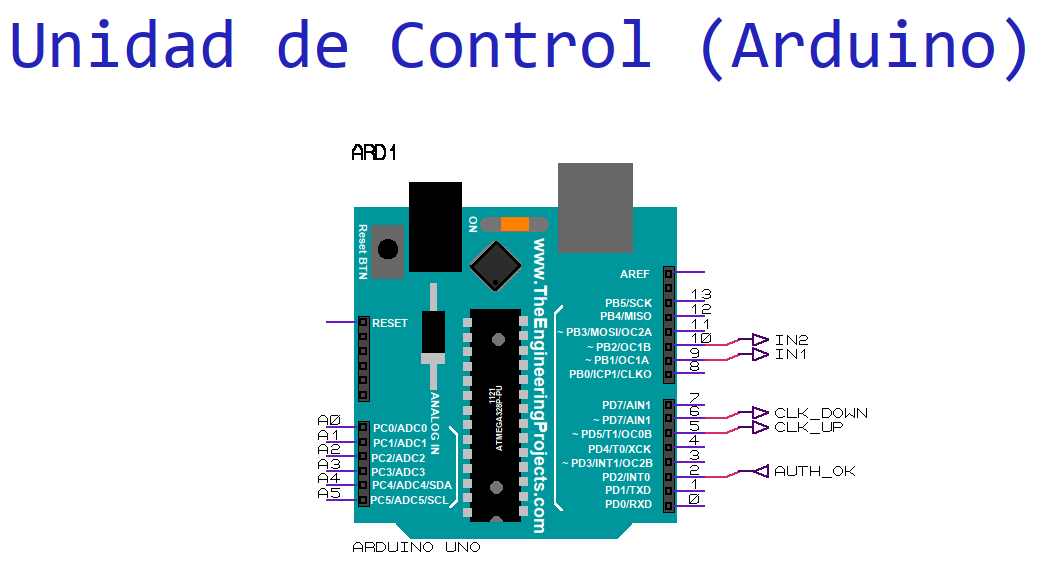
\includegraphics[width=0.55\textwidth]{assets/proteus_unidad_control_arduino.png}
    \caption{Unidad de control implementada con Arduino.}
\end{figure}

\subsection{Módulo de autenticación}
La autenticación se construyó en tres pasos: almacenamiento de contraseña, lectura del usuario y validación.

Primero, un 74LS174 almacena la contraseña definida por el grupo. Sus entradas provienen de un DIP switch de 4 bits y el botón \texttt{CLK\_MEM} funciona como pulso de memoria. El botón \texttt{RESET} limpia el registro y devuelve la contraseña a 0000. Esta decisión permitió que la contraseña quedara realmente memorizada en hardware y no en el microcontrolador.

Después, otro banco de interruptores define el valor ingresado por el usuario. Ambos buses se conectan a un 74LS85, que entrega la señal \texttt{MATCH} cuando los cuatro bits coinciden. Finalmente, un flip-flop 74LS74 toma \texttt{MATCH} en su entrada D y la memoriza cuando llega el pulso \texttt{VALIDATE}; por eso \texttt{AUTH\_OK} queda estable y no depende del tiempo exacto de presión del botón.

\begin{figure}[H]
    \centering
    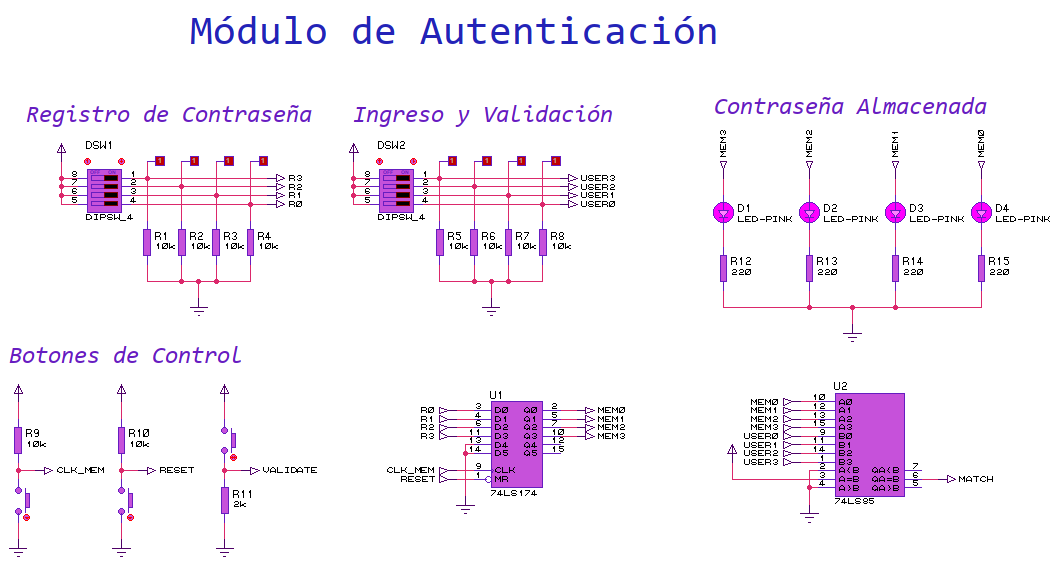
\includegraphics[width=\textwidth]{assets/proteus_modulo_autenticacion_general.png}
    \caption{Vista general del módulo de autenticación.}
\end{figure}

\begin{figure}[H]
    \centering
    \begin{subfigure}[t]{0.48\textwidth}
        \centering
        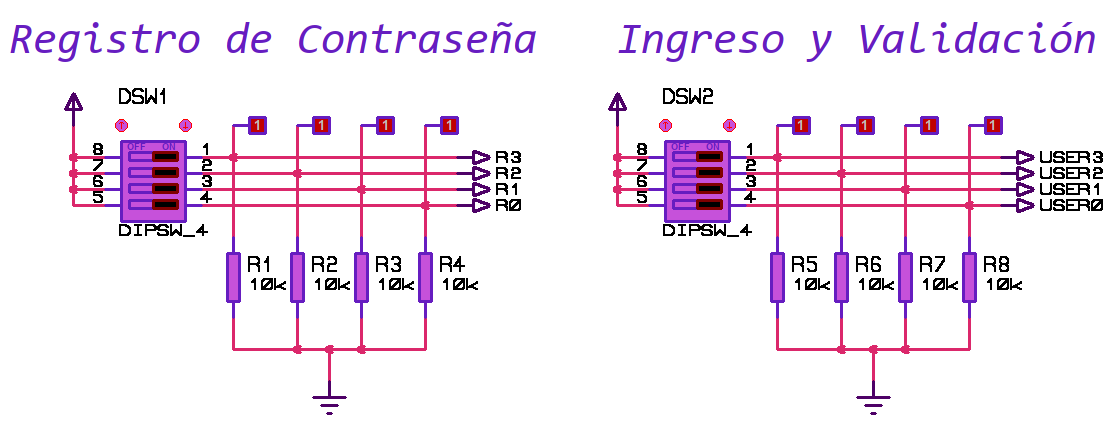
\includegraphics[width=\textwidth]{assets/proteus_registro_contrasena_ingreso_validacion.png}
        \caption{Bloque de registro e ingreso.}
    \end{subfigure}
    \hfill
    \begin{subfigure}[t]{0.48\textwidth}
        \centering
        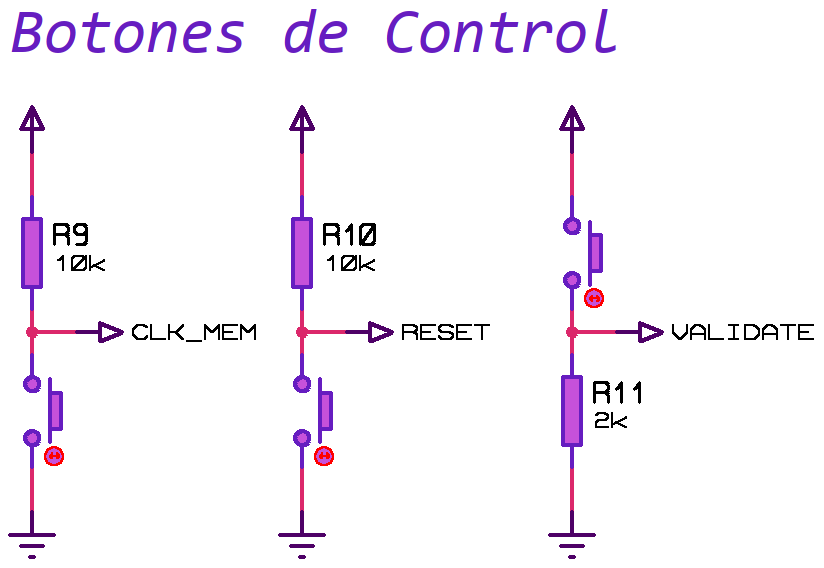
\includegraphics[width=\textwidth]{assets/proteus_botones_control.png}
        \caption{Botones de control.}
    \end{subfigure}
    \caption{Entradas manuales del sistema de autenticación.}
\end{figure}

\begin{figure}[H]
    \centering
    \begin{subfigure}[t]{0.48\textwidth}
        \centering
        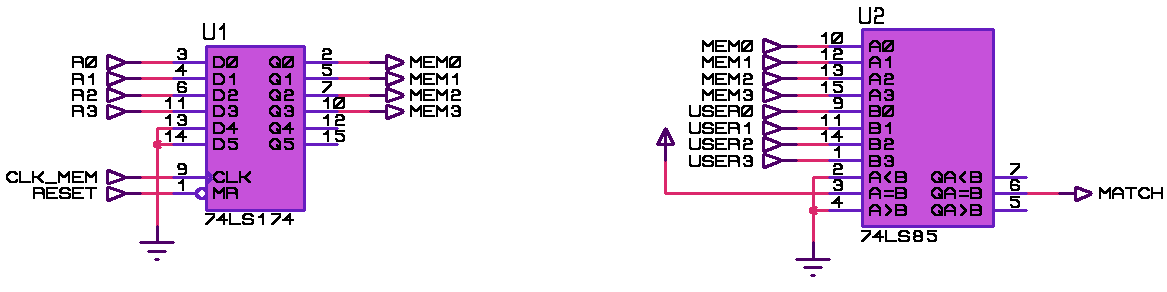
\includegraphics[width=\textwidth]{assets/proteus_memoria_contrasena_y_comparador.png}
        \caption{Registro 74LS174 y comparador 74LS85.}
    \end{subfigure}
    \hfill
    \begin{subfigure}[t]{0.48\textwidth}
        \centering
        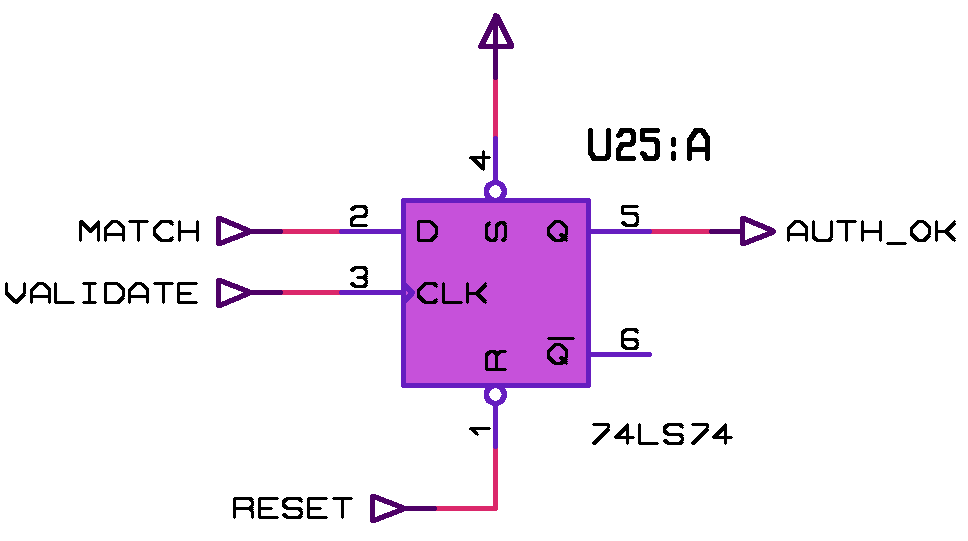
\includegraphics[width=\textwidth]{assets/proteus_latch_autorizacion_auth_ok.png}
        \caption{Latch de habilitación \texttt{AUTH\_OK}.}
    \end{subfigure}
    \caption{Implementación interna de memoria, comparación y validación.}
\end{figure}

\begin{figure}[H]
    \centering
    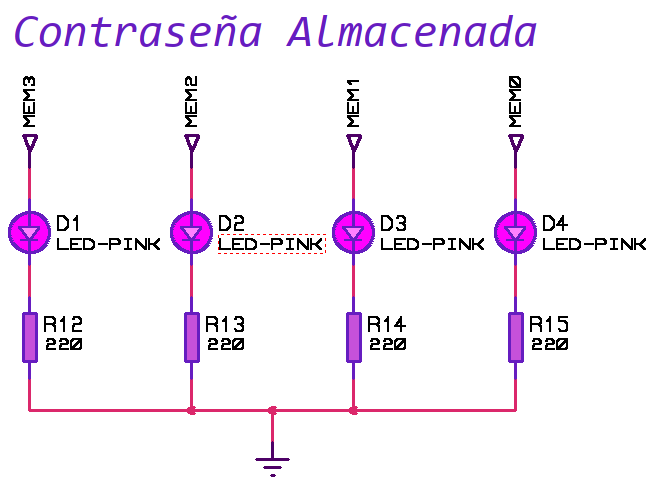
\includegraphics[width=0.65\textwidth]{assets/proteus_contrasena_almacenada_leds.png}
    \caption{LEDs que muestran visualmente la contraseña almacenada.}
\end{figure}

\subsection{Contador de errores y alarma}
Cada vez que el usuario presiona \texttt{VALIDATE} con una combinación incorrecta, la lógica genera un pulso \texttt{ERROR}. Ese pulso alimenta dos flip-flops tipo D en cascada, configurados como contador binario simple de dos bits. Su salida se conecta a un 74LS48 para mostrarse en un display de siete segmentos.

La elección de dos bits fue suficiente porque el sistema solo necesita distinguir los estados 0, 1, 2 y 3. Cuando el estado llega a 11, una compuerta AND genera \texttt{ALRM}; esa señal enciende un LED y un buzzer, e inmediatamente pasa por una inversora para producir \texttt{ENABLE = 0}. Con ello se bloquea la posibilidad de activar el movimiento hasta que se ingrese la contraseña correcta o se aplique el reinicio correspondiente.

\begin{figure}[H]
    \centering
    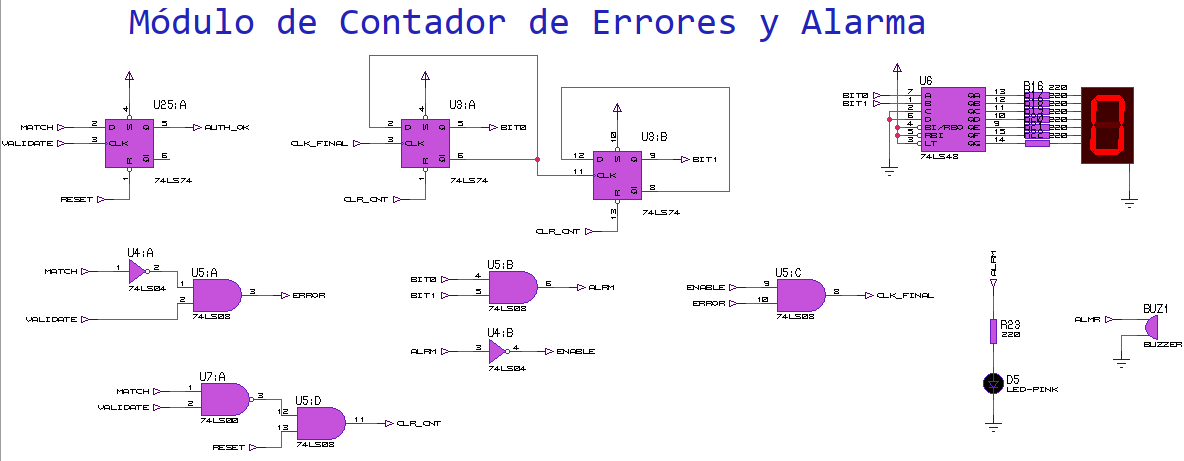
\includegraphics[width=\textwidth]{assets/proteus_modulo_contador_errores_alarma_general.png}
    \caption{Vista general del módulo de contador de errores y alarma.}
\end{figure}

\begin{figure}[H]
    \centering
    \begin{subfigure}[t]{0.48\textwidth}
        \centering
        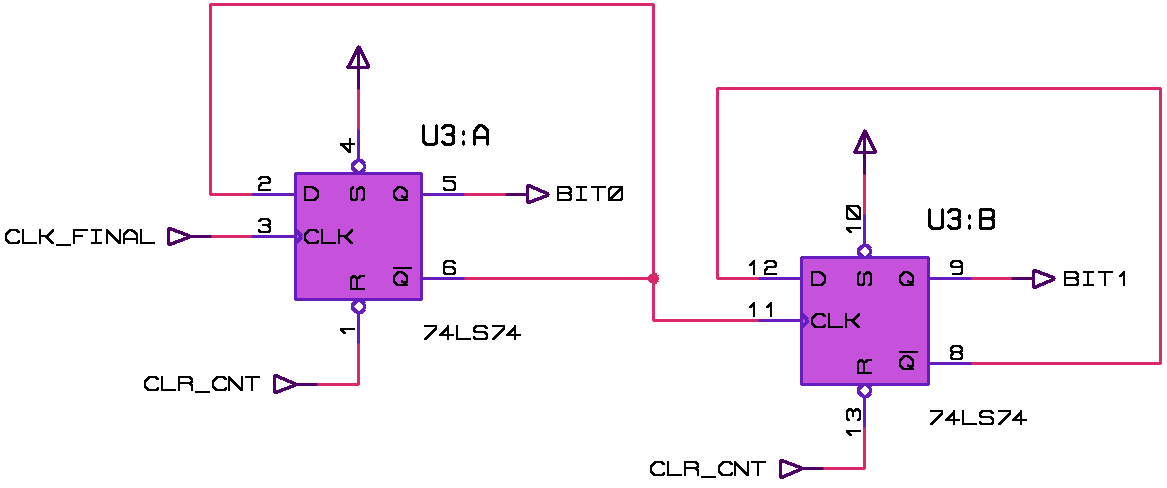
\includegraphics[width=\textwidth]{assets/proteus_contador_errores_flip_flops.png}
        \caption{Contador binario de errores con 74LS74.}
    \end{subfigure}
    \hfill
    \begin{subfigure}[t]{0.48\textwidth}
        \centering
        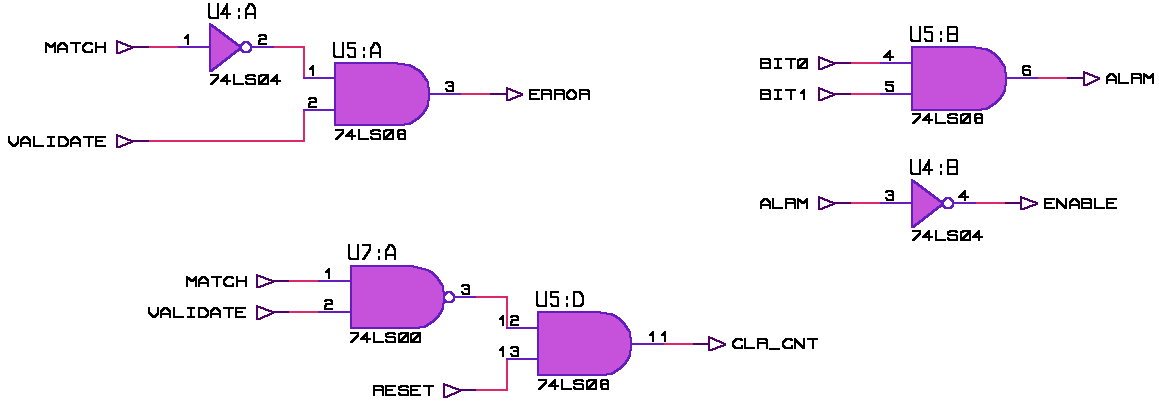
\includegraphics[width=\textwidth]{assets/proteus_logica_error_alarma_reset.png}
        \caption{Lógica de error, alarma y limpieza.}
    \end{subfigure}
    \caption{Construcción interna del módulo de seguridad.}
\end{figure}

\begin{figure}[H]
    \centering
    \begin{subfigure}[t]{0.42\textwidth}
        \centering
        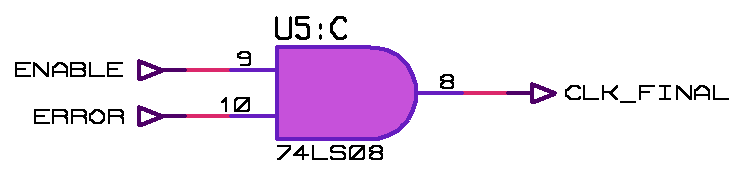
\includegraphics[width=\textwidth]{assets/proteus_display_contador_errores.png}
        \caption{Display del número de errores.}
    \end{subfigure}
    \hfill
    \begin{subfigure}[t]{0.42\textwidth}
        \centering
        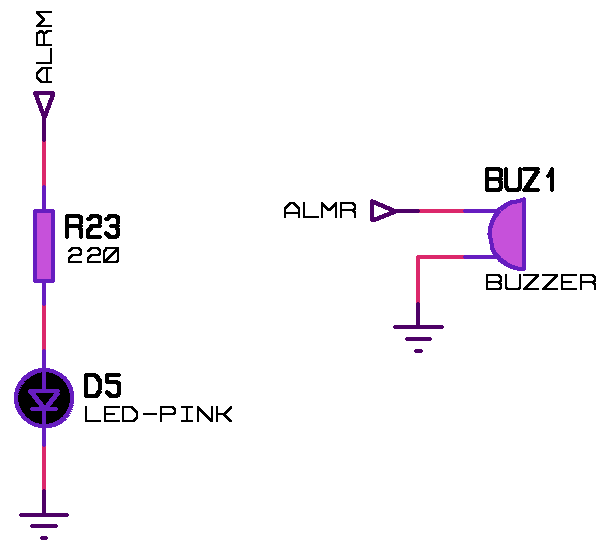
\includegraphics[width=\textwidth]{assets/proteus_indicadores_alarma_buzzer.png}
        \caption{Indicadores de alarma.}
    \end{subfigure}
    \caption{Elementos de salida del bloque de seguridad.}
\end{figure}

\subsection{Temporización y secuencia}
El módulo de temporización usa dos contadores distintos porque el enunciado exige dos comportamientos visuales: un conteo ascendente de 0 a 15 en la fase verde y un conteo descendente de 10 a 0 en la fase roja. Ambos contadores se implementaron con flip-flops tipo D, de modo que el proyecto mantuviera coherencia con la práctica y con la lógica secuencial vista en el curso.

El contador ascendente avanza una unidad por cada pulso de \texttt{CLK\_UP}. Además, incluye lógica para detectar cuándo el conteo ya superó 9, información que luego se usa para activar la decena del display. El contador descendente, por su parte, carga el valor 10 y después decrementa con cada pulso de \texttt{CLK\_DOWN}. La detección del estado 10 es importante porque al inicio de la fase roja deben mostrarse dos dígitos.

\subsubsection{Funcionamiento del contador ascendente}
El contador ascendente está formado por cuatro flip-flops tipo D conectados de manera que cada pulso de reloj hace avanzar el estado binario una unidad. El primer flip-flop representa el bit menos significativo y cambia en cada pulso; el segundo cambia cada dos pulsos; el tercero cada cuatro, y el cuarto cada ocho. En conjunto, esa estructura produce una cuenta natural de 0000 a 1111.

En términos prácticos, el comportamiento puede entenderse como una suma binaria de 1 en cada flanco de reloj:

\[
0000 \rightarrow 0001 \rightarrow 0010 \rightarrow 0011 \rightarrow \dots \rightarrow 1111
\]

Como 1111 en binario equivale a 15 en decimal, este bloque cubre exactamente la fase de 15 segundos pedida en el enunciado. Cada pulso generado por el Arduino representa un segundo, de modo que el display muestra el progreso de la fase verde desde 0 hasta 15. La lógica adicional conectada a las salidas detecta cuándo el conteo alcanzó valores mayores o iguales a 10 para activar la decena correspondiente en la visualización.

\begin{table}[H]
    \centering
    \caption{Secuencia representativa del contador ascendente.}
    \begin{tabular}{c c c}
        \toprule
        \textbf{Pulso} & \textbf{Estado binario} & \textbf{Valor decimal} \\
        \midrule
        Inicial & 0000 & 0 \\
        1 & 0001 & 1 \\
        2 & 0010 & 2 \\
        3 & 0011 & 3 \\
        4 & 0100 & 4 \\
        \dots & \dots & \dots \\
        10 & 1010 & 10 \\
        15 & 1111 & 15 \\
        \bottomrule
    \end{tabular}
\end{table}

\subsubsection{Funcionamiento del contador descendente}
El contador descendente también utiliza cuatro flip-flops tipo D, pero su lógica de realimentación no busca sumar uno, sino restar uno en cada pulso. Para evitar comenzar desde 1111, se incorporó una condición de carga que fuerza el valor inicial 1010, equivalente a 10 decimal. A partir de ahí, cada pulso de \texttt{CLK\_DOWN} hace que el conteo disminuya una unidad.

La secuencia principal del bloque es la siguiente:

\[
1010 \rightarrow 1001 \rightarrow 1000 \rightarrow 0111 \rightarrow \dots \rightarrow 0000
\]

Esta elección hace que el display muestre claramente el cierre de la segunda fase, ya que el tiempo restante va disminuyendo hasta llegar a cero. En el circuito puede verse una señal de detección del estado 10 y otra lógica auxiliar de carga; esto se utilizó para garantizar que el contador iniciara exactamente en 10 al arrancar la fase roja y no en otro valor residual.

\begin{table}[H]
    \centering
    \caption{Secuencia representativa del contador descendente.}
    \begin{tabular}{c c c}
        \toprule
        \textbf{Pulso} & \textbf{Estado binario} & \textbf{Valor decimal} \\
        \midrule
        Carga inicial & 1010 & 10 \\
        1 & 1001 & 9 \\
        2 & 1000 & 8 \\
        3 & 0111 & 7 \\
        4 & 0110 & 6 \\
        \dots & \dots & \dots \\
        9 & 0001 & 1 \\
        10 & 0000 & 0 \\
        \bottomrule
    \end{tabular}
\end{table}

\subsubsection{Relación entre contadores y secuencia del carrusel}
Los contadores no trabajan al mismo tiempo. Durante la fase verde, solo recibe pulsos el contador ascendente; el descendente permanece inactivo. Cuando termina la primera fase, el Arduino cambia la dirección del motor y comienza a enviar pulsos al contador descendente. Esa separación evita conflictos de visualización y hace que cada display represente de forma coherente el estado actual del carrusel.

Desde el punto de vista lógico, el sistema usa los contadores como memoria temporal del estado de la secuencia. No son únicamente un adorno visual: sus salidas participan en la detección de valores clave, como el paso a decenas o la carga del 10 inicial, y por eso forman parte del control general de la práctica.

\begin{figure}[H]
    \centering
    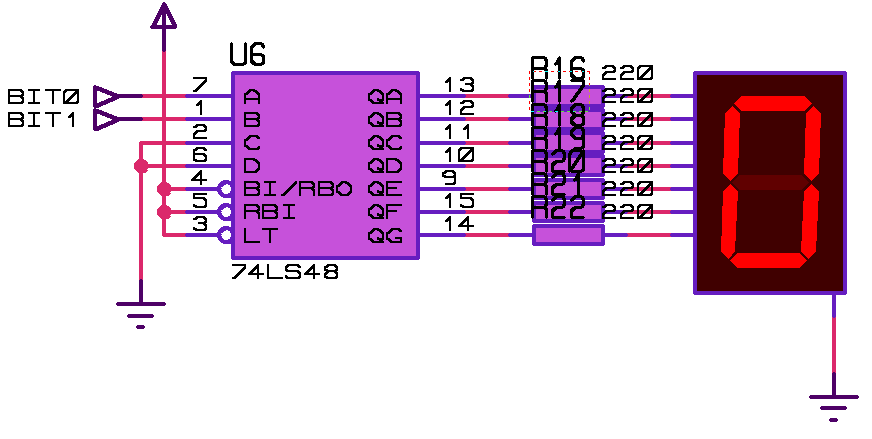
\includegraphics[width=0.8\textwidth]{assets/proteus_modulo_temporizacion_secuencia_general.png}
    \caption{Vista general del módulo de temporización y secuencia.}
\end{figure}

\begin{figure}[H]
    \centering
    \begin{subfigure}[t]{0.48\textwidth}
        \centering
        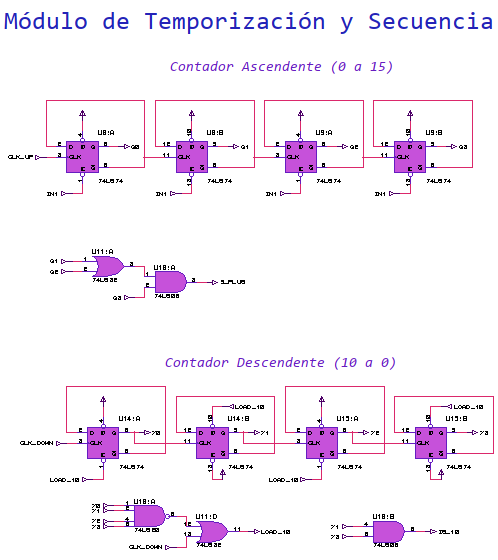
\includegraphics[width=\textwidth]{assets/proteus_contador_ascendente_0_a_15.png}
        \caption{Contador ascendente de 0 a 15.}
    \end{subfigure}
    \hfill
    \begin{subfigure}[t]{0.48\textwidth}
        \centering
        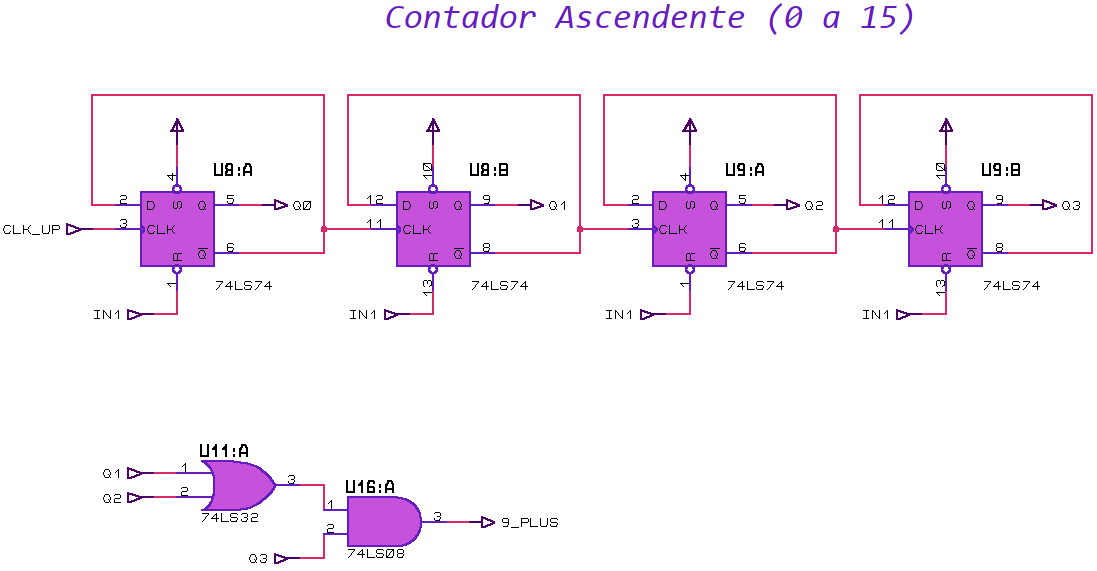
\includegraphics[width=\textwidth]{assets/proteus_contador_descendente_10_a_0.png}
        \caption{Contador descendente de 10 a 0.}
    \end{subfigure}
    \caption{Contadores empleados para las dos fases del carrusel.}
\end{figure}

\subsection{Multiplexación y displays de tiempo}
Una vez que ambos contadores existen, todavía hace falta decidir cuál de ellos será visible en los displays. Para eso se usaron multiplexores 74LS157. La lógica de selección entrega a la salida los bits del contador ascendente mientras el carrusel avanza, y conmuta a los bits del contador descendente durante la segunda fase.

También se agregó una etapa de ajuste BCD con un 74LS283 y un 74LS48. Esta sección evita que el display de las decenas permanezca siempre apagado: se enciende cuando el ascendente alcanza 10, 11, 12, 13, 14 o 15, y también al inicio del descendente cuando el valor es exactamente 10. Por eso el sistema puede mostrar valores de una y dos cifras sin cambiar la estructura principal de los contadores binarios.

\begin{figure}[H]
    \centering
    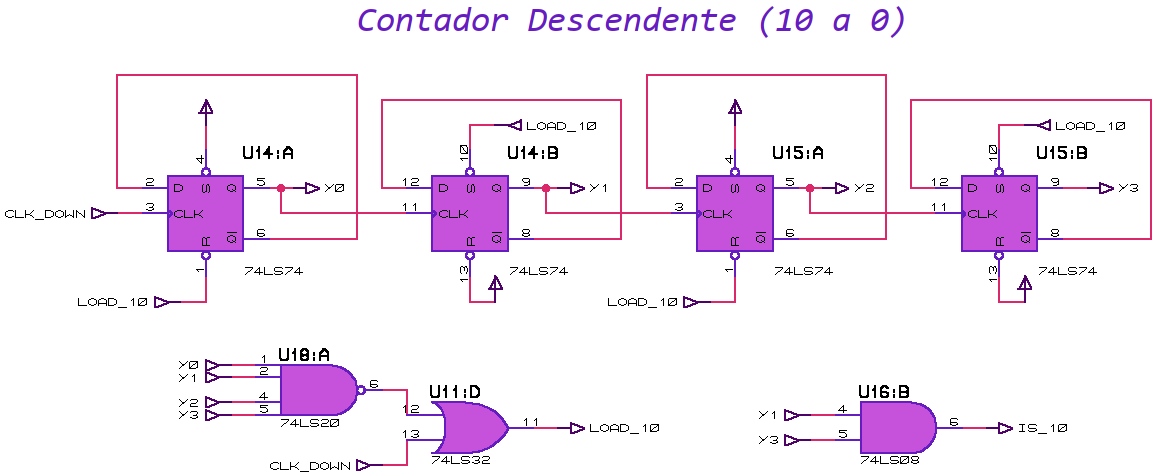
\includegraphics[width=\textwidth]{assets/proteus_logica_multiplexacion_y_displays_tiempo.png}
    \caption{Lógica de multiplexación y adaptación a displays de tiempo.}
\end{figure}

\subsection{Control del motor DC}
El motor del carrusel se controló mediante un puente H discreto con transistores 2N2222A y diodos 1N4007. Los diodos se colocaron para absorber los transitorios generados por la carga inductiva del motor, mientras que las entradas \texttt{IN1} e \texttt{IN2} determinan el sentido de circulación de corriente.

La implementación física muestra por qué separar este bloque fue útil: el motor y la maqueta mecánica generan vibraciones y variaciones de consumo, por lo que conviene que la lógica de autenticación y conteo permanezca aislada conceptualmente. Los LEDs verde y rojo se conectaron a las mismas líneas de control del sentido, de forma que el estado visual coincida con el estado eléctrico del puente H.

\begin{figure}[H]
    \centering
    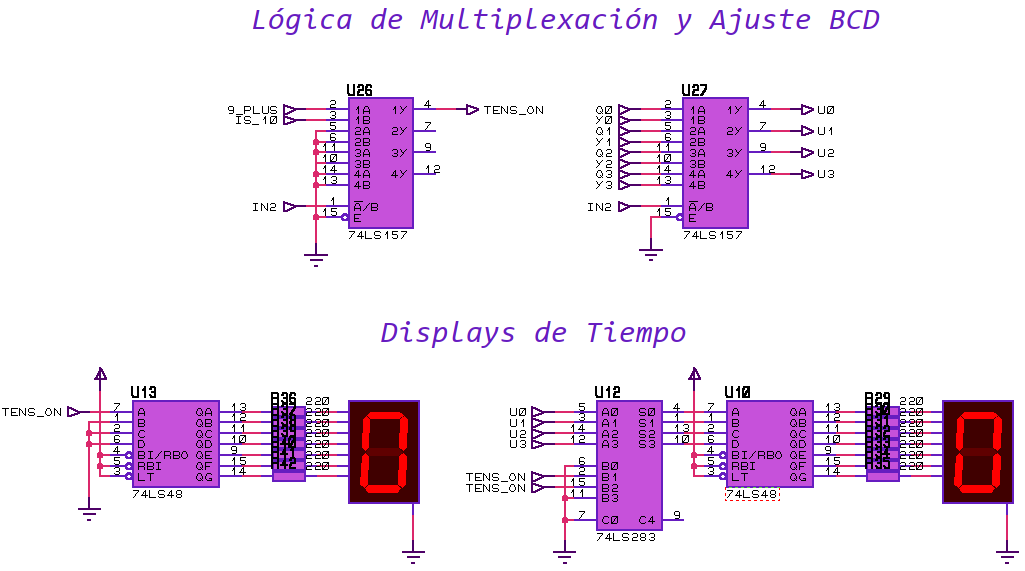
\includegraphics[width=0.9\textwidth]{assets/proteus_modulo_control_motor_dc_carrusel.png}
    \caption{Módulo de control del motor DC y señalización visual de giro.}
\end{figure}

\section{Diagramas del diseño del circuito}
En esta práctica se optó por documentar el diseño por módulos, ya que el circuito completo resulta extenso y menos legible cuando se presenta en una sola vista. Las capturas integradas en las secciones anteriores funcionan como diagramas técnicos del proyecto porque muestran cada subsistema con suficiente detalle para identificar entradas, salidas, compuertas de control, elementos de memoria y dispositivos de visualización.

La organización seguida en la documentación responde al flujo real del sistema. Primero se presenta la unidad de autenticación, porque ahí se origina la señal de habilitación general. Después se documenta el contador de errores, ya que depende del resultado de la validación y determina si el sistema puede continuar. A continuación se muestran los contadores temporizados y la lógica de multiplexación, que traducen la habilitación en una secuencia visible de tiempo. Finalmente, se expone el puente H y la etapa del motor, donde las señales digitales se convierten en movimiento físico del carrusel.

Este enfoque modular permite entender no solo cómo está cableado el proyecto, sino también por qué cada bloque fue implementado de esa forma. En lugar de presentar una sola captura saturada de conexiones, se privilegió una explicación progresiva: memoria, validación, seguridad, secuencia, visualización y potencia.

\section{Equipo utilizado}

\begin{table}[H]
    \centering
    \caption{Equipo y componentes principales empleados.}
    \small
    \begin{tabular}{p{4.5cm}p{2cm}p{7cm}}
        \toprule
        \textbf{Elemento} & \textbf{Cantidad} & \textbf{Uso en el proyecto} \\
        \midrule
        Arduino Uno & 1 & Generación de pulsos de reloj y control de dirección \\
        Protoboards grandes & 3 & Montaje de módulos lógicos y de potencia \\
        74LS174 & 1 & Registro de contraseña \\
        74LS85 & 1 & Comparación de contraseña de 4 bits \\
        74LS74 & 8 & Latches, contador de errores y contadores de tiempo \\
        74LS08 & 3 & Detección de estados y compuertas AND \\
        74LS32 & 2 & Compuertas OR auxiliares \\
        74LS04 & 1 & Inversión de señales de control \\
        74LS20 & 2 & Lógica NAND de limpieza y detección \\
        74LS157 & 2 & Multiplexación de la información visible \\
        74LS48 & 3 & Decodificación a display de siete segmentos \\
        74LS283 & 1 & Ajuste BCD para visualización de tiempo \\
        Displays de 7 segmentos & 3 & Tiempo y contador de errores \\
        DIP switches de 4 posiciones & 2 & Contraseña almacenada e ingreso del usuario \\
        Push buttons & 3 & Guardado, reinicio y validación \\
        LEDs & 6 & Indicadores de memoria, giro y alarma \\
        Resistencias de 220 $\Omega$ y 1 k$\Omega$ & Varias & Limitación de corriente y polarización \\
        Transistores 2N2222A & 4 & Puente H del motor \\
        Diodos 1N4007 & 4 & Protección ante retroceso del motor \\
        Motor DC con reducción & 1 & Movimiento del carrusel \\
        Cartón, palillos, impresión y decoración & Varios & Estructura física de la maqueta \\
        \bottomrule
    \end{tabular}
\end{table}

\section{Presupuesto estimado}
No se contó con una factura consolidada de todo el proyecto, por lo que el presupuesto se construyó a partir de los costos reportados por los integrantes del grupo. En los casos en que no se entregó factura individual, el valor se consigna como gasto reportado.

\begin{table}[H]
    \centering
    \caption{Presupuesto reportado del proyecto.}
    \small
    \begin{tabular}{p{5.2cm}r r r}
        \toprule
        \textbf{Componente} & \textbf{Cantidad} & \textbf{Unitario (Q)} & \textbf{Subtotal (Q)} \\
        \midrule
        Arduino Uno & 1 & 150.00 & 150.00 \\
        Motor DC & 1 & 19.00 & 19.00 \\
        74LS174 & 1 & 10.00 & 10.00 \\
        74LS74 & 2 & 8.00 & 16.00 \\
        Buzzer activo 5V & 1 & 5.00 & 5.00 \\
        Resistencias de 10 k$\Omega$ & 10 & 0.75 & 7.50 \\
        4 transistores y 4 diodos & 1 lote & 16.00 & 16.00 \\
        Gasto reportado por otros integrantes & 1 lote & 68.00 & 68.00 \\
        \midrule
        \textbf{Total reportado} &  &  & \textbf{291.50} \\
        \bottomrule
    \end{tabular}
\end{table}

\section{Fotografías del equipo y de la maqueta}
Las siguientes fotografías muestran el ensamblado físico del proyecto. En ellas puede observarse la separación práctica entre el bloque mecánico del carrusel, la lógica cableada sobre protoboard y la zona de pruebas del motor y del sistema de autenticación.

\begin{figure}[H]
    \centering
    \begin{subfigure}[t]{0.47\textwidth}
        \centering
        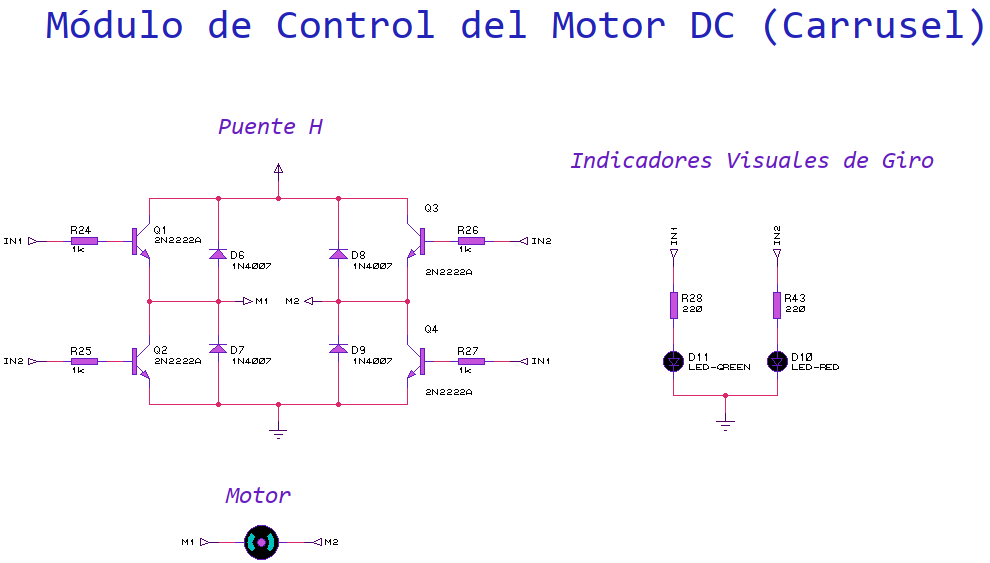
\includegraphics[width=\textwidth]{assets/armado_fisico_carrusel_maqueta_completa.jpeg}
        \caption{Maqueta completa con carrusel, Arduino y bancos de protoboard.}
    \end{subfigure}
    \hfill
    \begin{subfigure}[t]{0.47\textwidth}
        \centering
        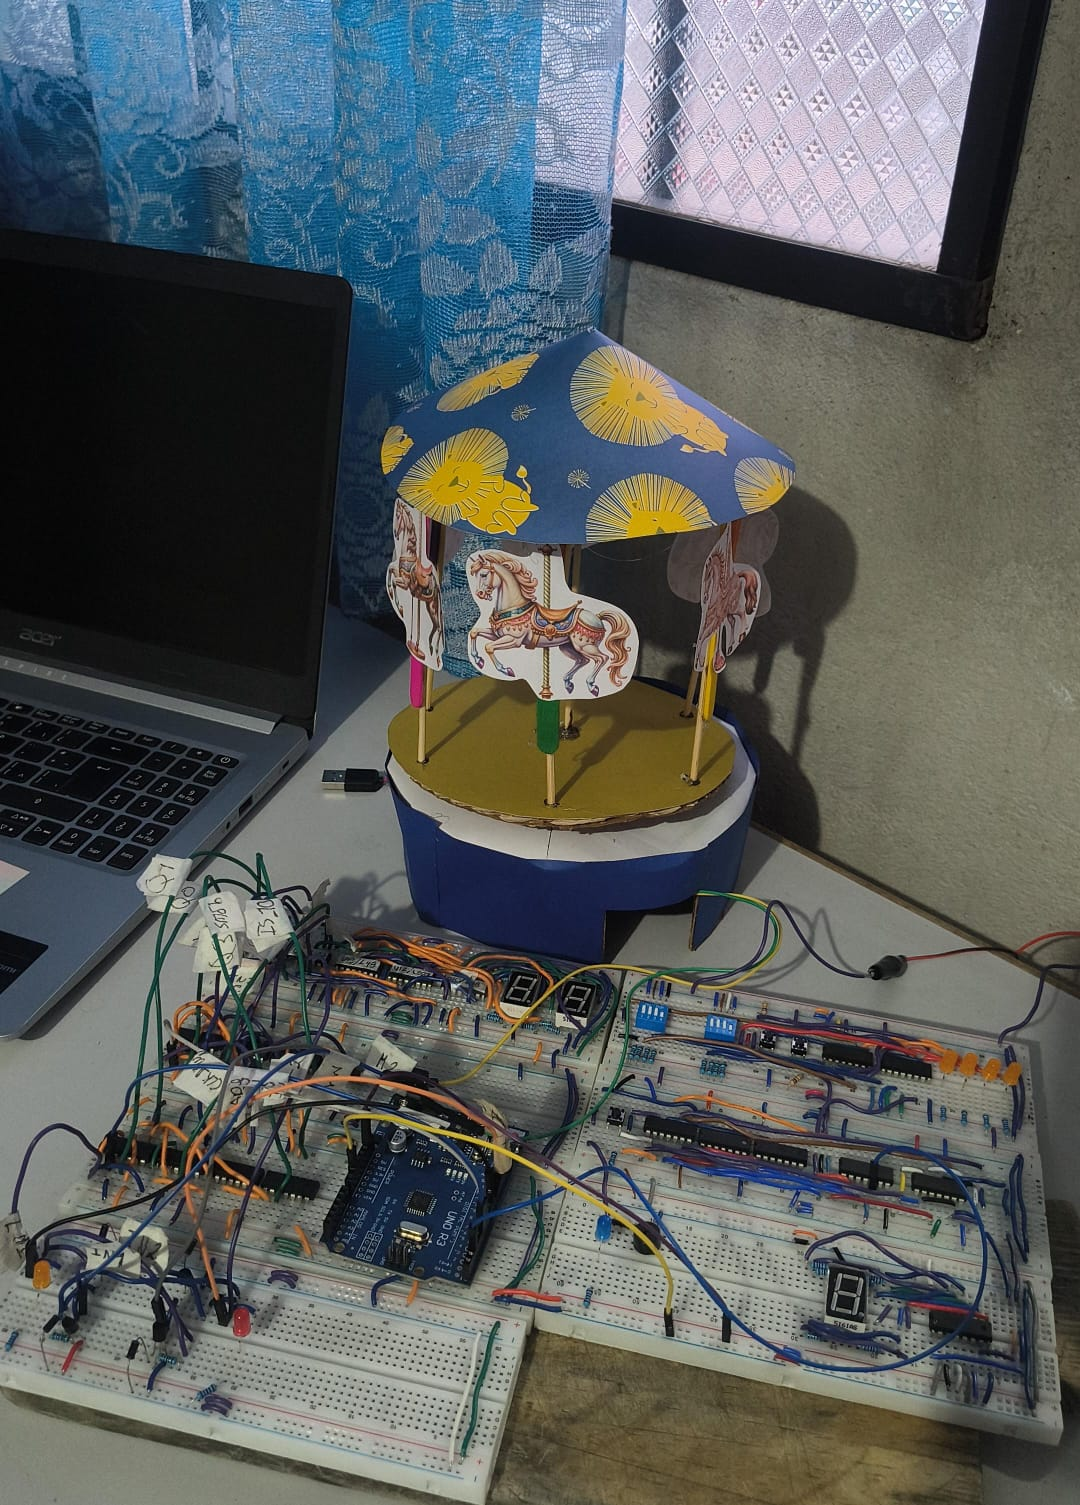
\includegraphics[width=\textwidth]{assets/armado_fisico_carrusel_con_breadboards.jpeg}
        \caption{Integración física del carrusel con las placas de control.}
    \end{subfigure}
    \caption{Vistas generales del montaje final.}
\end{figure}

\begin{figure}[H]
    \centering
    \begin{subfigure}[t]{0.47\textwidth}
        \centering
        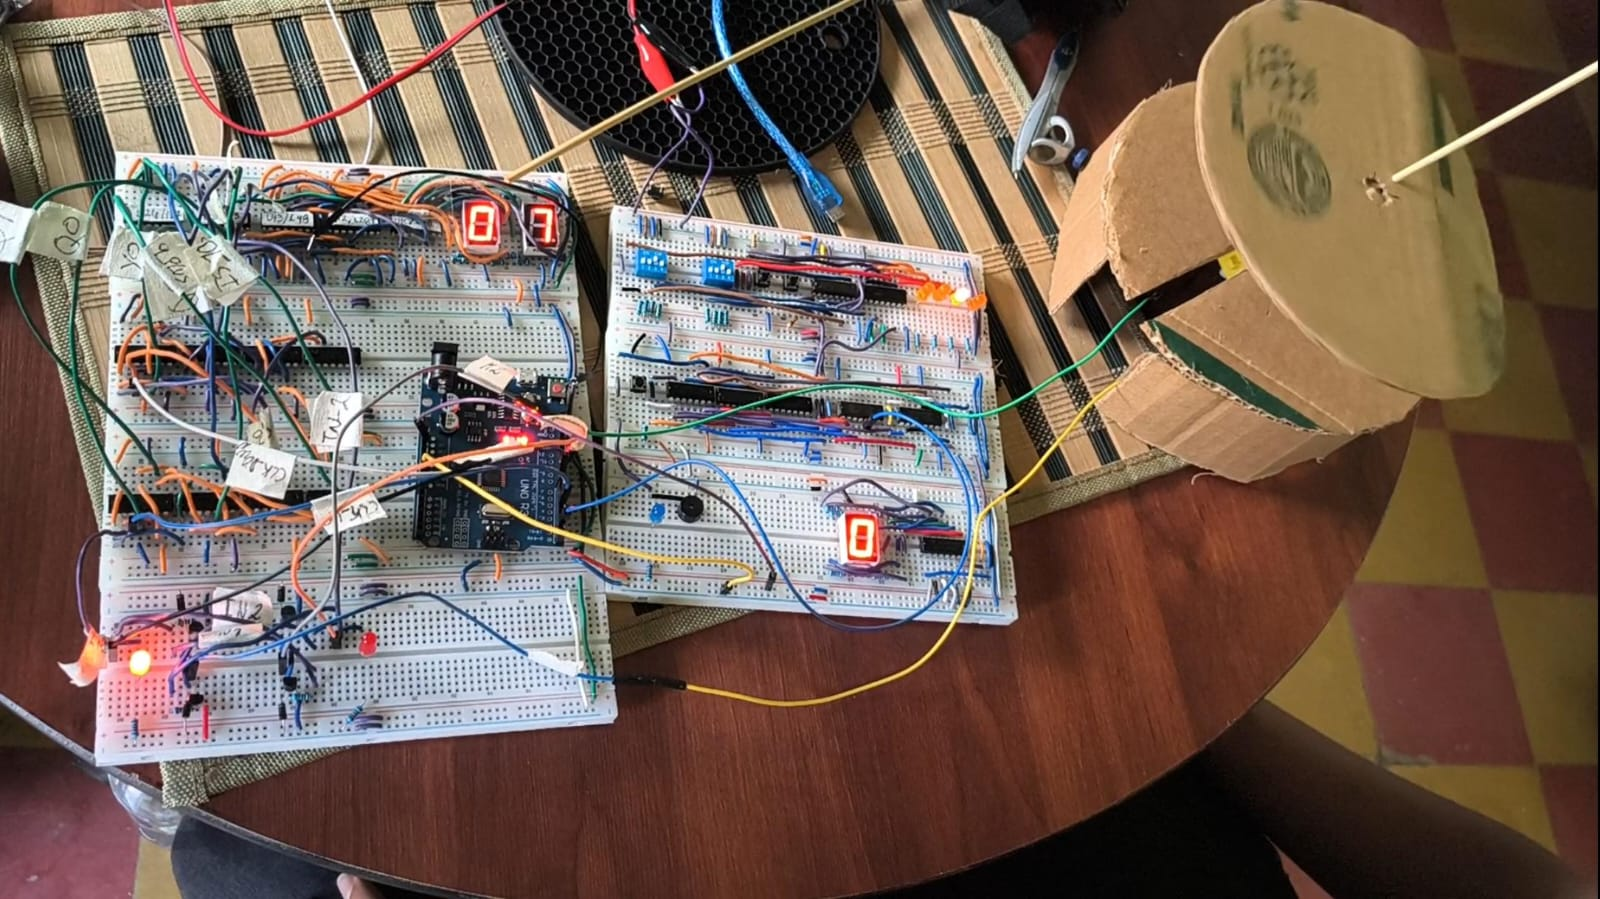
\includegraphics[width=\textwidth]{assets/armado_fisico_carrusel_vista_superior.jpeg}
        \caption{Vista superior durante pruebas de funcionamiento.}
    \end{subfigure}
    \hfill
    \begin{subfigure}[t]{0.32\textwidth}
        \centering
        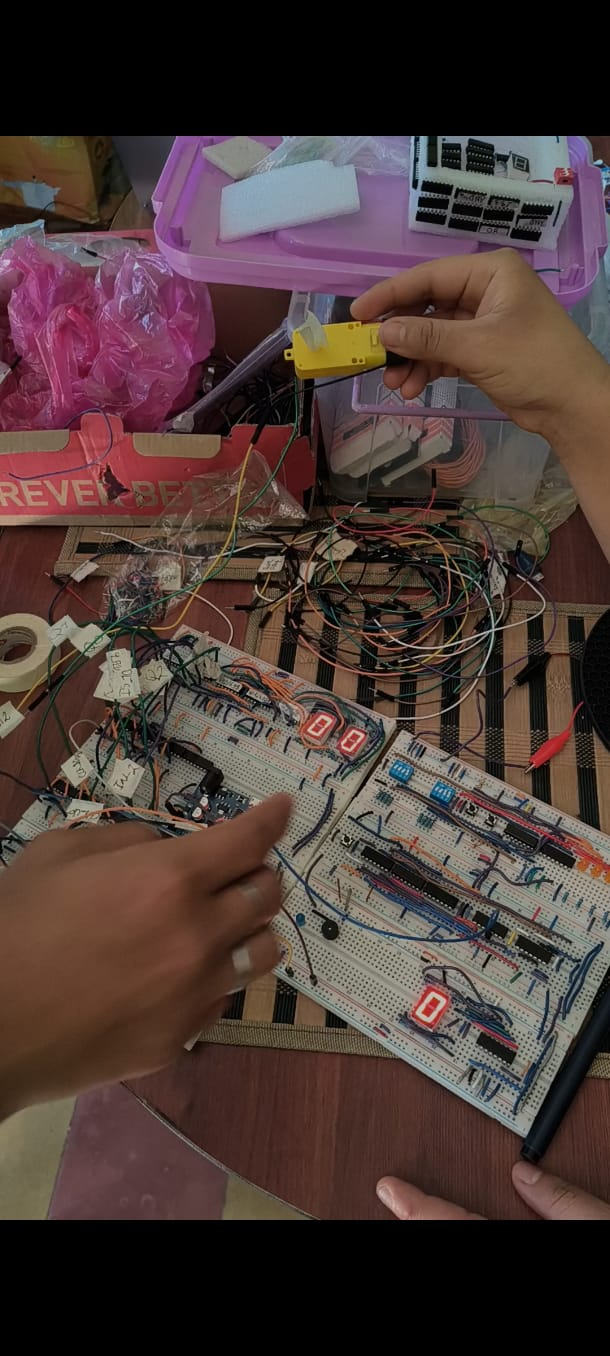
\includegraphics[width=\textwidth]{assets/armado_fisico_prueba_motor_y_cableado.jpeg}
        \caption{Prueba del motor y ajuste del cableado.}
    \end{subfigure}
    \caption{Evidencia del proceso de armado y validación.}
\end{figure}

\section{Análisis del funcionamiento}
El circuito muestra una separación clara de responsabilidades. La autenticación está aislada del movimiento; esto evita que una perturbación en la etapa de potencia altere la memoria de la contraseña o el conteo de errores. Asimismo, el uso de un latch para \texttt{AUTH\_OK} resuelve un problema frecuente en este tipo de prácticas: si la señal de coincidencia dependiera solo del botón o del comparador en tiempo real, el sistema podría arrancar y detenerse de forma errática por rebotes o por variaciones manuales en los switches.

El contador de errores también está bien planteado desde el punto de vista didáctico. En lugar de usar un contador dedicado, se construyó con flip-flops D, lo cual obliga a razonar sobre estados, limpieza y detección del valor límite. La alarma basada en el estado 3 es simple, pero suficiente para el requerimiento del enunciado y fácil de verificar visualmente tanto en la simulación como en el montaje.

En la parte temporal, la decisión de usar dos contadores diferentes hace más clara la presentación del tiempo. Un contador ascendente representa correctamente el progreso de la primera fase y un descendente comunica mejor el cierre de la segunda. Luego, la multiplexación unifica ambas salidas para no duplicar demasiados displays y mantiene una interfaz visual más ordenada. Finalmente, el puente H permite invertir físicamente el giro del motor y lo conecta con la lógica de estado mediante los LEDs rojo y verde, logrando correspondencia directa entre lo que el circuito decide y lo que el usuario observa.

Desde el punto de vista constructivo, las fotografías muestran que el mayor reto no fue solo la lógica, sino la integración. El proyecto combina elementos mecánicos, cableado extenso, varias familias TTL y un motor con consumo propio. Por ello, el orden del montaje, la identificación de señales y la separación física por módulos fueron decisiones necesarias para que la maqueta pudiera operar de manera estable y comprensible durante la demostración.

\section{Conclusiones}
\begin{itemize}[leftmargin=1.2cm]
    \item Se implementó un sistema de acceso seguro funcional usando lógica secuencial y combinacional, sin delegar la comparación de contraseña al Arduino.
    \item El contador de errores y la alarma cumplen el objetivo de bloquear el sistema tras tres intentos fallidos consecutivos y restablecer la operación solo con autenticación válida.
    \item La secuencia de 15 segundos de avance y 10 segundos de retorno quedó separada del bloque de seguridad, lo cual simplificó el diseño y la depuración.
    \item La documentación por módulos resulta más legible que una sola vista completa del circuito, especialmente en una práctica que mezcla registro, temporización, visualización y potencia.
    \item La maqueta física evidencia que el proyecto no se quedó en simulación: fue necesario ajustar cableado, distribución en protoboard y montaje mecánico para lograr una demostración integrada.
\end{itemize}

\end{document}
